\section{Numerical Results}
\begin{frame}{Approximation of Coupled Shear Flow Problem}
	\scriptsize
	Consider
	\begin{equation}
		\begin{split}
			&\partial_t Q(x,t) + A\partial_x Q(x,t) =  D(w_x)Q(x,t)+ D_rEQ(x,t) \\
			&\partial_{t}w = \partial_{xx}w + \delta(\bar{\rho}-2\sqrt{\pi} c^0_0(x,t)).
		\end{split}
		\label{coupledsys_1d}
	\end{equation}
	\begin{table}[h]
		\centering
		\renewcommand{\arraystretch}{1.3}
		\scalebox{0.95}{
			\begin{tabular}{|c|l|}
				\hline
				1. & $\frac{1}{2} \Delta t$ step on $\partial_t Q(x, t) = (D(w_x(x,t_n))+ D_rE)Q(x,t)$ \\
				\hline
				2. & $\frac{1}{4} \Delta t$ step on $\partial_t w(x, t) = \delta(\bar{\rho} - 2\sqrt{\pi} c^0_0(x,t))$ \\
				3. & $\frac{1}{2} \Delta t$ step on $\partial_t w(x, t) = \partial_{xx} w(x, t)$ \\
				4. & $\frac{1}{4} \Delta t$ step on $\partial_t w(x, t) = \delta(\bar{\rho} -2\sqrt{\pi} c^0_0(x,t))$ \\
				\hline
				5. & $\Delta t$ step on $\partial_t Q(x, t) + A \partial_x Q(x, t) = 0$ \\
				\hline
				6. & $\frac{1}{4} \Delta t$ step on $\partial_t w(x, t) = \delta(\bar{\rho} - 2\sqrt{\pi} c^0_0(x,t))$ \\
				7. & $\frac{1}{2} \Delta t$ step on $\partial_t w(x, t) = \partial_{xx} w(x, t)$ \\
				8. & $\frac{1}{4} \Delta t$ step on $\partial_t w(x, t) = \delta(\bar{\rho} -2\sqrt{\pi} c^0_0(x,t))$ \\
				\hline
				9. & $\frac{1}{2} \Delta t$ step on $\partial_t Q(x, t) = (D(w_x(x,t_{n+1}))+ D_rE)Q(x,t)$ \\
				\hline
			\end{tabular}
		}
		\caption{Splitting algorithm for solving the coupled shear flow problem (Dahm et al.)}
	\end{table}
	We use an ODE solver for $1.+9.$, LeVeque’s high resolution wave propagation algorithm for $5.$ and finite difference methods for the evolution of $w$.
\end{frame}


%----------------------------------------------------------

\begin{frame}{Coupled Problems}
	\begin{itemize}
		\item externally imposed velocity field \checkmark
		\item \textcolor{gray}{1D shear flow} \checkmark
         \item \textcolor{gray}{2D rectilinear flow \checkmark}
         \item \textcolor{gray}{3D flow with periodic boundary conditions}
	\end{itemize}
\end{frame}

\begin{frame}{Numerical Result for externally imposed velocity field}
		\scriptsize
		\begin{figure}[H]
			\centering
			\begin{minipage}{0.45\textwidth}
				\includegraphics[scale=0.3]{Bilder_wx/wx=1_Dr=0.1_N=7}
			\end{minipage}
			\hfill 
			\begin{minipage}{0.45\textwidth}
				\includegraphics[scale=0.3]{Bilder_wx/wx=1_Dr=1_N=7}
			\end{minipage}
			\caption{Numerical solution of the drift-diffusion term with constant externally imposed velocity gradient corresponding to shear flow using different values of $D_r$.}	
		\end{figure}
\end{frame}

\begin{frame}{Numerical Result for externally imposed velocity field}
	\scriptsize
	\begin{figure}[H]
	\centering
	 \begin{minipage}{0.4\textwidth}
	 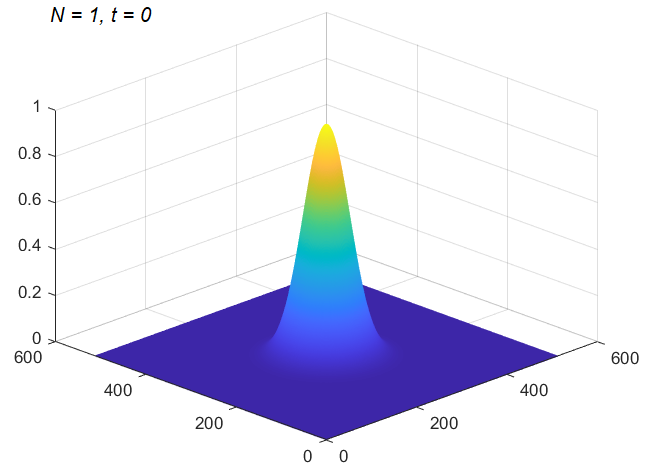
\includegraphics[scale=0.3]{Bilder_wxwy/t=0_wxwy=1_wxwy=-1}
     \end{minipage}
     \hfill 
     \begin{minipage}{0.4\textwidth}
	   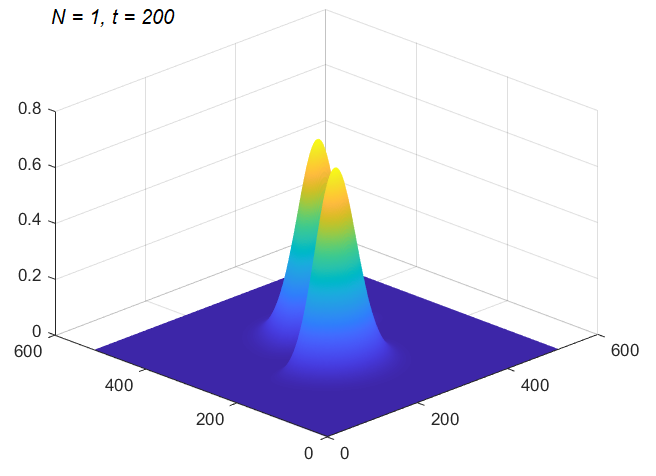
\includegraphics[scale=0.3]{Bilder_wxwy/t=200_wxwy=1_wxwy=-1}
     \end{minipage}
     \caption{Numerical results for $c^0_0$ at different times using $D_r=1$ and $w_x=w_y=1$ for $x<50$ and $w_x=w_y=-1$ otherwise. A cluster with higher particle density splits into two, each moving in opposite directions.}
    \end{figure}
\end{frame}



%----------------------------------------------------------
\begin{frame}{Coupled Problems}
	\begin{itemize}
		\item externally imposed velocity field \checkmark
		\item 1D shear flow \checkmark
		\item \textcolor{gray}{2D rectilinear flow \checkmark}
		\item \textcolor{gray}{3D flow with periodic boundary conditions}
	\end{itemize}
\end{frame}

\begin{frame}{Numerical Result for Shear Flow}
		\scriptsize
		Let 
		\begin{align*}
			c^0_0 (x,0) = (1+(1\cdot10^{-4} \cdot \eta(x)-5\cdot10^{-5}))/(2\sqrt{\pi}),
		\end{align*}
		where $\eta(x)$ is a random variable taking values in the interval $\pm \frac{1}{2}$.
		
		\begin{figure}
			\centering
			\begin{minipage}{0.46\textwidth}
				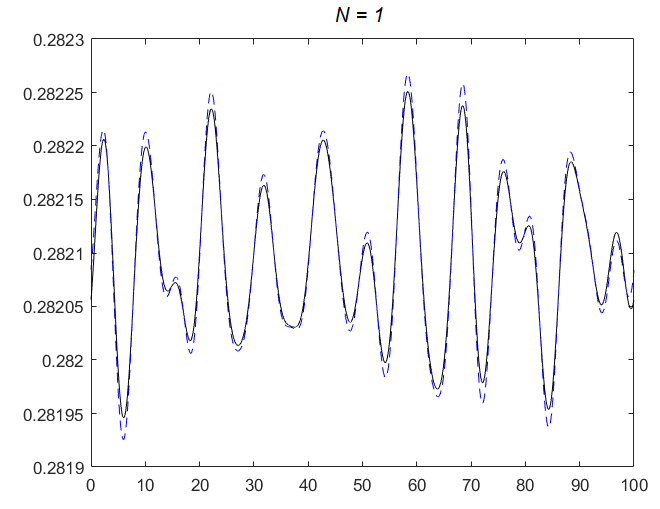
\includegraphics[width=\textwidth]{Bilder_wx/ClusterFormation/N=1vsN=6_Dr=0.05_mx=8192}
			\end{minipage}
			\hfill
			\begin{minipage}{0.46\textwidth}
				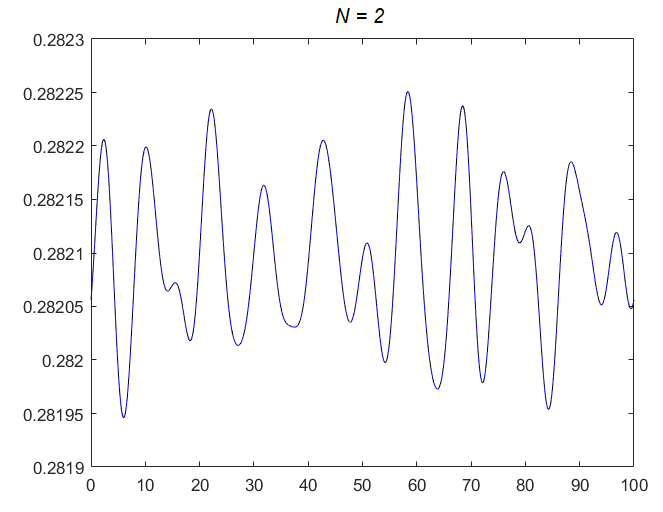
\includegraphics[width=\textwidth]{Bilder_wx/ClusterFormation/N=2vsN=6_Dr=0.05_mx=8192}
			\end{minipage}
			\caption{Approximation of the coupled problem for shear flow with $D_r =0.05$. The plot shows the density at time $t=30$ for $N = 1$ and $N = 2$ (blue line). A reference solution is calculated with $N = 6$ moment equations (black line).}
			\label{ClusterFormation}
		\end{figure}
		%The Figure (\ref{ClusterFormation}) shows that using $N = 1$ moment equations, compared to the reference solution with $N = 6$, already provides a good approximation of cluster formation. The numerical solution for $N=2$ aligns very well with the reference solution.
\end{frame}


%----------------------------------------------------------

\begin{frame}{Coupled Problems}
	\begin{itemize}
		\item externally imposed velocity field \checkmark
		\item 1D shear flow \checkmark
		\item 2D rectilinear flow \checkmark
		\item \textcolor{gray}{3D flow with periodic boundary conditions}
	\end{itemize}
\end{frame}

\begin{frame}
	\scriptsize
	\begin{figure}[H]
		\begin{minipage}{0.4\textwidth}
			\centering
			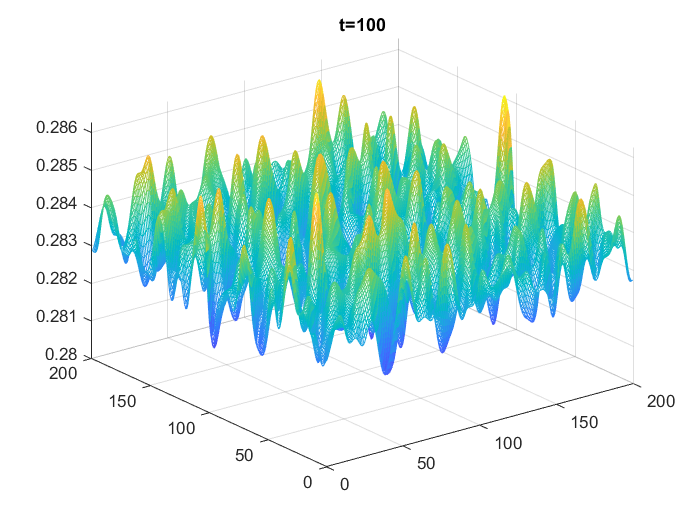
\includegraphics[scale=0.25]{Bilder_wxwy/2nd_t=100_mx=my=200_random_Dr=1_(1.d0+(1.d-2rand(0)-5.d-4))Divide(2.d0dsqrt(pi))}
		\end{minipage}
		\hfill 
		\begin{minipage}{0.4\textwidth}
			\centering
			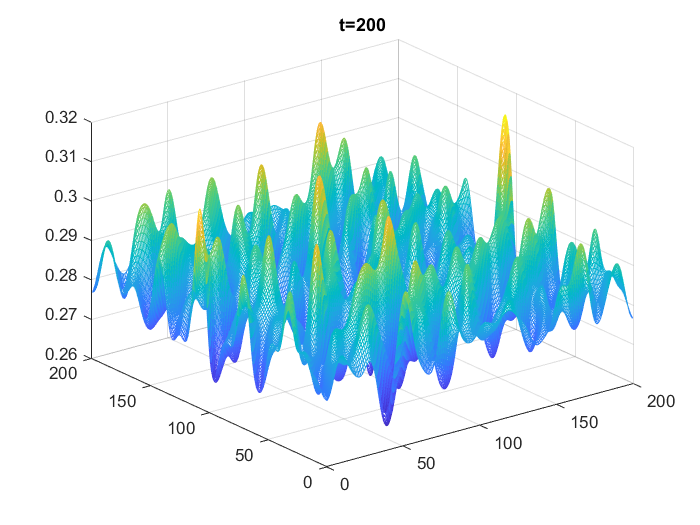
\includegraphics[scale=0.25]{Bilder_wxwy/2nd_t=200_mx=my=200_random_Dr=1_(1.d0+(1.d-2rand(0)-5.d-4))Divide(2.d0dsqrt(pi))}
		\end{minipage}
		
		\vspace{1ex}
		\centering
		Solution structure of \(c^0_0\) with \(N = 1\).
		
		\vspace{2ex}
		
		\begin{minipage}{0.4\textwidth}
			\centering
			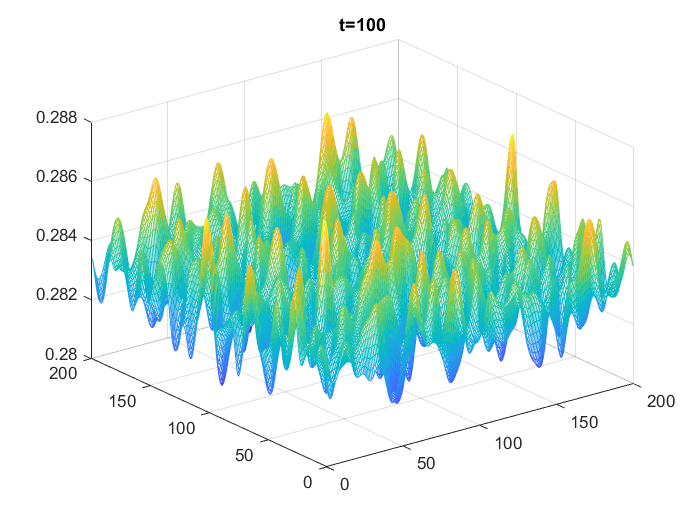
\includegraphics[scale=0.25]{Bilder_wxwy/14th_t=100_mx=my=200_random_Dr=1_(1.d0+(1.d-2rand(0)-5.d-4))Divide(2.d0dsqrt(pi))}
		\end{minipage}
		\hfill 
		\begin{minipage}{0.4\textwidth}
			\centering
			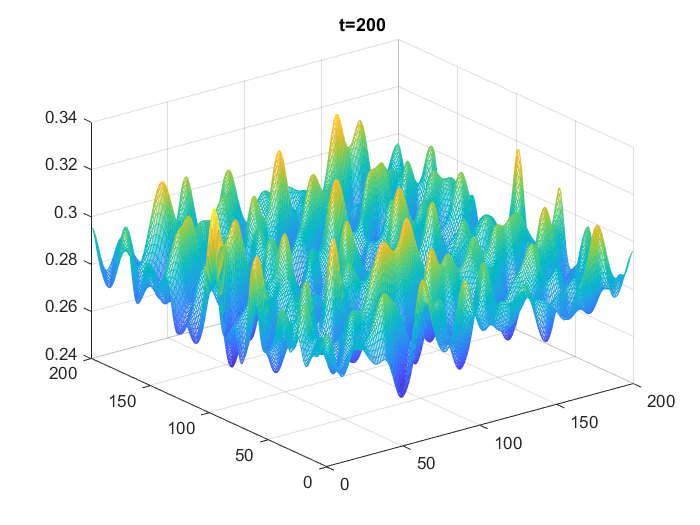
\includegraphics[scale=0.25]{Bilder_wxwy/14th_t=200_mx=my=200_random_Dr=1_(1.d0+(1.d-2rand(0)-5.d-4))Divide(2.d0dsqrt(pi))}
		\end{minipage}
		
		\caption{Solution structure of \(c^0_0\) with \(N = 7\).}
	\end{figure}
\end{frame}



